%
%===============>>  ГРУППА 6-1 МОДУЛЬ 6  <<=============
%
\setmodule{6}

%BEGIN_FOLD % ====>>_____ Занятие 1 _____<<====
\begin{class}[number=1]
	\begin{listofex}
		\item
		\begin{minipage}[t]{\bodywidth}
			Определите координаты точек:
		\end{minipage}
		%\hspace{0.02\linewidth}
		\begin{minipage}[c]{0.45\textwidth}
			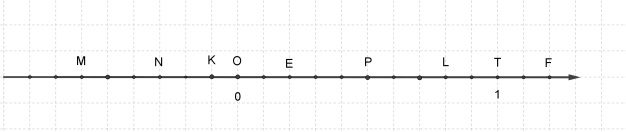
\includegraphics[align=t, width=\linewidth]{\picpath/G61M6L1-1}
		\end{minipage}
	\end{listofex}
		\begin{definit}
			Чтобы вычесть из отрицательного числа отрицательное число, нужно сложить их так, будто они положительные, а перед суммой поставить минус.
		\end{definit}
	\begin{listofex}[resume]
		\item Вычислите:
		\begin{tasks}(4)
			\task \( -28-14 \)
			\task \( -144-56 \)
			\task \( -9-17 \)
			\task \( -3-18 \)
			\task \( -12-7 \)
			\task \( -15-8 \)
			\task \( -24-19 \)
			\task \( -8-3 \)
		\end{tasks}
	\end{listofex}
		\begin{definit}
			Для удобства, при сложении отрицательного числа с положительным, сумму можно записать как разность, поставив положительное число перед отрицательным. \\ Например, \(-12+25=25-12=13\).
		\end{definit}
	\begin{listofex}[resume]
		\item Вычислите:
		\begin{tasks}(4)
			\task \( -35 + 92 \)
			\task \( -7+14 \)
			\task \( -17+21 \)
			\task \( -5+65 \)
			\task \( -26+27 \)
			\task \( -8+12 \)
			\task \( -32+32 \)
			\task \( -80+124 \)
		\end{tasks}
	\end{listofex}
		\begin{definit}
			Если перед скобками стоит знак минус, то при их раскрытии знак внутри скобок меняется на противоположный. \\ Например: \(-(-a) = a \) или \( -(b) = -b \)
		\end{definit}
	\begin{listofex}[resume]
		\item Вычислите:
		\begin{tasks}(3)
			\task \( -35 - (-42) \)
			\task \( 8-(6) \)
			\task \( -(19)-(-21) \)
			\task \( -5-(-27) \)
			\task \( -(-42)+18 \)
			\task \( -(-17)-26 \)
			\task \( -(-29)+(-13) \)
			\task \( -(18)+(-12) \)
		\end{tasks}
	\end{listofex}
		\begin{definit}
		Чтобы из меньшего числа вычесть большее, необходимо из большего вычесть меньшее и перед результатом поставить знак минус. \\ Например: \( 17-82 = -(82-17)=-65 \)
		\end{definit}
	\begin{listofex}[resume]
		\item Вычислите:
		\begin{tasks}(4)
			\task \( 15-21 \)
			\task \( 17-66 \)
			\task \( 100-143 \)
			\task \( 42-69 \)
			\task \( 85-98 \)
			\task \( 117-162 \)
			\task \( 31-67 \)
			\task \( 71-143 \)
		\end{tasks}
		\item Вычислите:
		\begin{tasks}(2)
			\task \( -\mfrac{2}{3}{7}-\mfrac{3}{5}{14} \)
			\task \( -\mfrac{4}{8}{9}+\mfrac{6}{7}{15} \)
			\task \( -3,3+\mfrac{4}{8}{7} \)
			\task \( -5,6+\mfrac{5}{3}{5} \)
			\task \( 9,9-\mfrac{11}{4}{15} \)
			\task \( -\mfrac{8}{4}{23}+\mfrac{9}{5}{46}+\left(-\mfrac{18}{13}{69}\right) \)
			\task \( -2,3 + \left(-\mfrac{1}{3}{5}\right) + 9,09 \)
			\task \( -\mfrac{6}{8}{12} + \left(-\dfrac{13}{24}\right) - (-7,11) \)
		\end{tasks}
	\end{listofex}
\end{class}
%END_FOLD

%BEGIN_FOLD % ====>>_____ Занятие 2 _____<<====
\begin{class}[number=2]
	\begin{listofex}
		\item
		\begin{minipage}[t]{\bodywidth}
			Определите координаты всех точек:
		\end{minipage}
		%\hspace{0.02\linewidth}
		\begin{minipage}[c]{0.45\textwidth}
			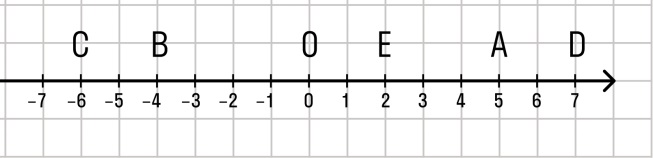
\includegraphics[align=t, width=\linewidth]{\picpath/G61M6L2-1}
		\end{minipage}
	\end{listofex}
	\begin{definit}
		Рациональные числа, как и целые, можно сравнивать с помощью числовой оси --- \textbf{чем правее расположено число, тем оно больше.}
	\end{definit}
	\begin{listofex}[resume]
		\item С помощью этого же рисунка сравните координаты точек:
		\begin{tasks}(3)
			\task \( A \) и \( D \)
			\task \( B \) и \( C \)
			\task \( B \) и \( E \)
			\task \( O \) и \( B \)
			\task \( E \) и \( C \)
			\task \( O \) и \( C \)
		\end{tasks}
		\item Сравните рациональные числа:
		\begin{tasks}(3)
			\task \( -5 \) и \( -3 \)
			\task \( -7 \) и \( -25 \)
			\task \( 4 \) и \( -1 \)
			\task \( -99 \) и \( -101 \)
			\task \( -10,5 \) и \( -1,5 \)
			\task \( -8,9 \) и \( -9,2 \)
			\task \( -55,3 \) и \( -55,4 \)
			\task \( -0,2 \) и \( 0 \)
			\task \( \dfrac{1}{3} \) и \( -\dfrac{1}{4} \)
			\task \(- \dfrac{4}{7} \) и \( \dfrac{3}{4} \)
			\task \(- \mfrac{1}{3}{15} \) и \( -\dfrac{3}{15} \)
			\task \( -\mfrac{2}{3}{4} \) и \( -\dfrac{2}{5} \)
		\end{tasks}
		\item Вычислите:
		\begin{tasks}(3)
			\task \( -\dfrac{5}{9}-\dfrac{5}{9} \)
			\task \( -\dfrac{14}{15}+\dfrac{5}{6} \)
			\task \( -\dfrac{1}{2}-\dfrac{1}{3} \)
			\task \( \mfrac{3}{5}{6}-4 \)
			\task \( -1,18+\dfrac{33}{50} \)
			\task \( -0,8+4 \)
			\task \( 1,7-7,3 \)
			\task \( -2,4+3,6 \)
			\task \( -5,7-2,15 \)
		\end{tasks}
		\item У нас было  \(115\)  рублей, в первом магазине потратили \(\dfrac{2}{5}\) этой суммы истратили, а потом еще \(\dfrac{8}{10}\) от остатка. Сколько денег мы потратили и сколько денег у нас осталось?
		\item В четырех домах \(567\) жителя. В одном доме \(\dfrac{1}{3}\) всех жителей, во втором --- в \(1,5\) раза меньше, чем в первом, а остальные живут поровну в третьем и четвёртом домах. По скольку жителей живёт в третьем и четвёртом домах?
		\item Из одного центра управления запущены три беспилотника для видеосъемки акватории Азовского моря. Время съемки первого --- \(8\) мин, второго --- \(12\) мин, а третьего --- \(18\) мин. Через какое время беспилотники одновременно вернуться в центр управления, если их запускают вновь после очередной перезарядки?
		\item Решите пропорции:
		\begin{tasks}(2)
			\task \( \dfrac{x}{24}=\dfrac{15}{6} \)
			\task \( 14:x=5:8\)
		\end{tasks}
	\end{listofex}
\end{class}
%END_FOLD

%BEGIN_FOLD % ====>>_ Домашняя работа 1 _<<====
\begin{homework}[number=1]
	\begin{listofex}
		\item Вычислите:
		\begin{tasks}(2)
			\task \( -11 + 21 \)
			\task \( -17+25 \)
			\task \( -37+65 \)
			\task \( -51-14 \)
			\task \( -26-37 \)
			\task \( -83-22 \)
			\task \( -\dfrac{1}{3}+\dfrac{1}{2} \)
			\task \( -\mfrac{2}{1}{6}+11 \)
			\task \( -1,5-\dfrac{3}{7} \)
			\task \( -\mfrac{3}{5}{21}+\mfrac{3}{17}{42}+\left(-\mfrac{18}{45}{66}\right) \)
			\task \( -15,2 + \left(-\mfrac{2}{17}{25}\right) + 12 \)
			\task \( -\mfrac{4}{2}{3} + \left(-\dfrac{22}{24}\right) - (-6) \)
		\end{tasks}
		\item Сравните рациональные числа:
		\begin{tasks}(3)
			\task \( -\dfrac{1}{2} \) и \( -\dfrac{3}{4} \)
			\task \( -\dfrac{5}{11} \) и \( -\dfrac{6}{33} \)
			\task \( -\mfrac{1}{5}{7} \) и \( -\dfrac{13}{8} \)
			\task \( -11,5 \) и \( -17,22 \)
			\task \( -8,85 \) и \( -8,02 \)
			\task \( -14,4 \) и \( -14,02 \)
		\end{tasks}
	\end{listofex}
\end{homework}
%END_FOLD

%BEGIN_FOLD % ====>>_____ Занятие 3 _____<<====
\begin{class}[number=3]
	\begin{definit}
		Противоположные числа --- это числа, которые в алгебраической сумме дают значение ноль. \\
		\begin{minipage}[c]{0.45\textwidth}
			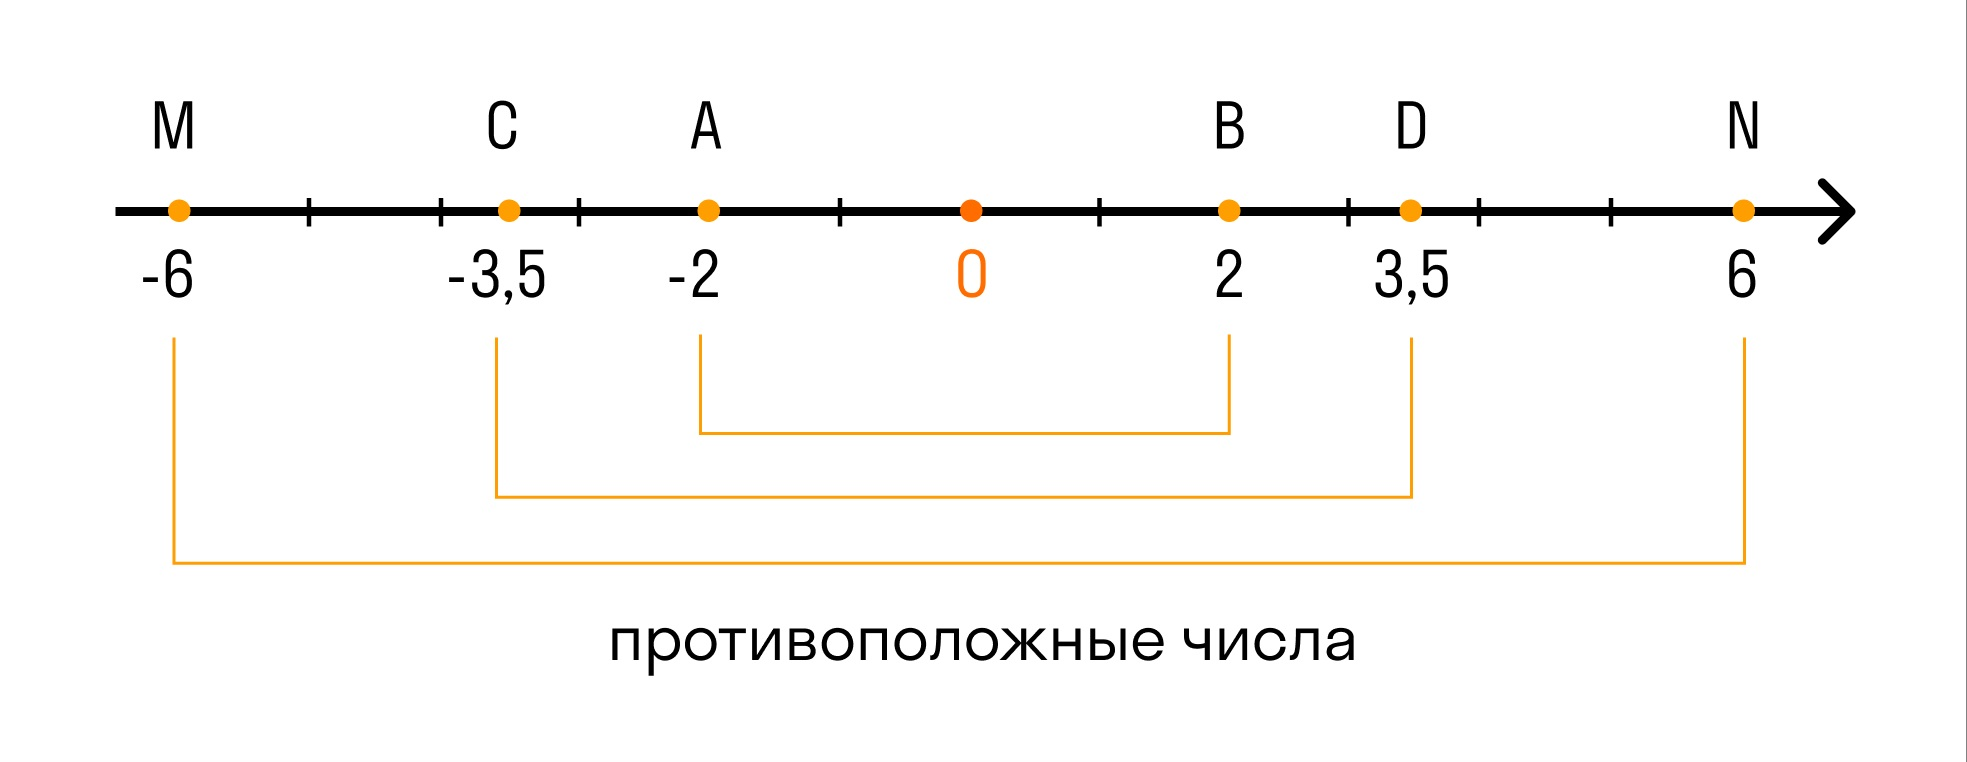
\includegraphics[align=t, width=\linewidth]{\picpath/G61M6L3-1}
		\end{minipage}
	\end{definit}
	\begin{listofex}
		\item Запишите число, противоположное данному:
		\begin{tasks}(4)
			\task \( -11  \)
			\task \( 25 \)
			\task \( 0,16 \)
			\task \( -26 \)
			\task \( 55,11 \)
			\task \( \dfrac{-2}{3} \)
			\task \( \dfrac{22}{-3} \)
			\task \( -\dfrac{5}{(-12)} \)
		\end{tasks}
		\item Найдите сумму чисел, противоположных данным:
		\begin{tasks}(4)
			\task \( -15  \) и \( 21 \)
			\task \( -7  \) и \( -5,5 \)
			\task \( 12  \) и \( 66,2 \)
			\task \( -31  \) и \( -0,22 \)
			\task \( -\dfrac{3}{4}  \) и \( 1,2 \)
			\task \( -\dfrac{5}{12}  \) и \( -\mfrac{3}{5}{6} \)
			\task \( -\dfrac{3}{7}  \) и \( \mfrac{5}{9}{14} \)
		\end{tasks}
	\end{listofex}
	\begin{definit}
	Модулем положительного числа называется само число. \\
	Модулем отрицательного числа называется противоположное ему число. \\
	Модуль нуля равен нулю.
	\end{definit}
	\begin{listofex}[resume]
		\item Найдите модуль:
		\begin{tasks}(3)
			\task \(  |3| \)
			\task \(  |-15| \)
			\task \( |-14+52|  \)
			\task \( |-17-5,7|  \)
			\task \(  \left|2-\mfrac{4}{5}{6}\right| \)
			\task \(  \left|\dfrac{-1}{4}\right| \)
			\task \(  \left|\dfrac{-8}{15}\right| \)
			\task \(  \left|-\mfrac{7}{8}{9} - \left|-\dfrac{27}{9}\right|\right| \)
		\end{tasks}
		\item Вычислите:
		\begin{tasks}(2)
			\task \(  |-5|+|-11| \)
			\task \(  -|-15|-|11,5| \)
			\task \( |-21+32| - \left|\dfrac{-3}{5}\right|  \)
			\task \( -|-9|+|15-7,3|-|-25|  \)
			\task \(  |-4,5|-\left|-\mfrac{2}{1}{2}\right| \)
			\task \(  -\left| \dfrac{-5}{8} \right|-\left|\dfrac{-3}{4}\right| \)
			\task \(  \left|\dfrac{-8}{15}\right| + \bigl|-3,5+|-12,2|| \)
			\task \(  \left|-\mfrac{3}{5}{6} - \left|-4+\dfrac{16}{9}\right|\right| \)
		\end{tasks}
		\item Запишите без скобок:
		\begin{tasks}(3)
			\task \( -(-9) \)
			\task \( -(-10) \)
			\task \( -(-(-57)) \)
			\task \( -(-(-(-0,1))) \)
			\task \( -(-a) \)
			\task \( -(-(-a)) \)
			\task \( -(-(-(-(-a)))) \)
			\task \( \underbrace{-(-(-...}_{57}a)) \)
			\task \( \underbrace{-(-(-...}_{2022}a)) \)
		\end{tasks}
		\item Известно, что \( |a|<|b| \). Как могут быть расположены на числовой прямой числа \( a \) и \( b \). Перечислите все возможные случаи. Схематично изобразите все случаи на числовой прямой.
		\item Гонщик проехал сначала \(30\%\) трассы, а потом \(0,4\) метров оставшейся части трассы. После этого длина оставшейся части трассы стала равна \(210\) м. Сколько метров составляет длина трассы?
	\end{listofex}
\end{class}
%END_FOLD

%BEGIN_FOLD % ====>>_____ Занятие 4 _____<<====
\begin{class}[number=4]
	\begin{listofex}
		\item Для данного числа укажите модуль и противоположное число:
		\begin{tasks}(4)
			\task \( 6 \)
			\task \( -57 \)
			\task \( -5 \)
			\task \( \dfrac{1}{3} \)
			\task \( -\mfrac{5}{11}{13} \)
			\task \( -2,557 \)
			\task \( -\mfrac{3}{5}{7} \)
			\task \( -0,98 \)
		\end{tasks}
		\item Найдите значение выражения:
		\begin{tasks}(2)
			\task \( |-8|-|-5| \)
			\task \( |-2,3|+|3,7|  \)
			\task \(  |-10|\cdot|-15| \)
			\task \( |-4,7|-|-1,9| \)
			\task \( \left|\dfrac{7}{9}\right|-\left|-\mfrac{1}{2}{3}\right| \)
			\task \( |-4|\cdot\left|-\mfrac{1}{3}{4}\right| \)
			\task \( \left|\mfrac{2}{3}{14}-\mfrac{1}{5}{7}\right|-\left|\dfrac{19}{21}\right| \)
			\task \( -\left|\mfrac{2}{5}{16}-\dfrac{17}{8}\right|+\left|-\dfrac{5}{4}\right| \)
		\end{tasks}
		\item Найдите сумму модулей двух чисел:
		\begin{tasks}(3)
			\task \( -15 \) и \( 5,8 \)
			\task \( 7 \) и \( -17 \)
			\task \( -\dfrac{2}{3} \) и \( 12,5 \)
			\task \( -\dfrac{5}{6} \) и \( -\mfrac{1}{5}{12} \)
			\task \( -7,5 \) и \( -\dfrac{1}{3} \)
			\task \( 3,4 \) и \( -\mfrac{2}{3}{5} \)
		\end{tasks}
		\item Вычислите:
		\begin{tasks}(2)
			\task \( -12 + 31 \)
			\task \( -15+11 \)
			\task \( -6+8,8 \)
			\task \( -7,3-14 \)
			\task \( -15-\dfrac{2}{4} \)
			\task \( -|11,1|+\mfrac{2}{3}{4} \)
			\task \( -\dfrac{1}{3}-\dfrac{1}{2} \)
			\task \( -\mfrac{2}{1}{6}-\left|-\mfrac{7}{5}{6}\right| \)
			\task \( -1,5-\dfrac{3}{7} \)
			\task \( -\mfrac{4}{8}{11}+\left|-\mfrac{2}{17}{21}\right|+\left(-\mfrac{3}{5}{11}\right) \)
			\task \( |-1,2| + \left(-\mfrac{2}{17}{25}\right) - |-12| \)
			\task \( -\mfrac{5}{1}{4} + \left(-\dfrac{3}{8}\right) - \left|-\mfrac{1}{5}{7}-\dfrac{11}{14}\right| \)
		\end{tasks}
		\item Решите уравнения:
		\begin{tasks}(2)
			\task \( -x=607 \)
			\task \( -a=30,4 \)
			\task \( -y=-57 \)
			\task \( -y=-\mfrac{3}{15}{16} \)
			%\task \( -t=0 \)
			%\task \( -b=-5,67 \)
			%\task \( -x=-0,01 \)
			%\task \( x-=-0,02 \)
			%\task \( -b=-5,7 \)
			%\task \( -a=-\dfrac{5}{7} \)
		\end{tasks}
		\item В одном бассейне было в \(3\) раза больше воды, чем в другом. Когда из каждого бассейна выкачали по \(200\) м\(^3\) воды, во втором осталось в \(5\) раз меньше воды, чем в первом. Сколько кубических метров воды было в каждом бассейне первоначально?
	\end{listofex}
\end{class}
%END_FOLD

%BEGIN_FOLD % ====>>_ Домашняя работа 2 _<<====
\begin{homework}[number=2]
	\begin{listofex}
		\item Запишите число, противоположное данному:
		\begin{tasks}(4)
			\task \( 56  \)
			\task \( -12 \)
			\task \( -0,9 \)
			\task \( -33 \)
			\task \( 125,2 \)
			\task \( -\dfrac{2}{3} \)
			\task \( \dfrac{1}{-5} \)
			\task \( -\dfrac{(-7)}{-15} \)
		\end{tasks}
		\item Найдите сумму чисел, противоположных данным:
		\begin{tasks}(4)
			\task \( -7  \) и \( 5 \)
			\task \( -1,5  \) и \( 0,12 \)
			\task \( \dfrac{5}{8}  \) и \( -\mfrac{2}{3}{16} \)
			\task \( -\dfrac{1}{3}  \) и \( -\mfrac{5}{4}{9} \)
		\end{tasks}
		\item Вычислите:
		\begin{tasks}(2)
			\task \(  |-3|+|-5| \)
			\task \( |-11|-|21|-|-25|  \)
			\task \(  |-15,2|-\left|-\mfrac{5}{13}{25}\right| \)
			\task \(  -\left|\dfrac{-18}{9}\right| + |-7,5-|-1,2|| \)
		\end{tasks}
		\item Вычислите: \[ -\dfrac{13}{-4} + \left(-\dfrac{3}{8}\right) - \left|-\mfrac{3}{5}{8}+\dfrac{1}{16}\right| \]
		\item В первой бутылке было в \(4\) раза больше оливкового масла, чем во второй. Когда из первой бутылки перелили во вторую \(1,6\) л, то во второй бутылке стало в \(1,5\) раза больше масла, чем в первой. Сколько литров масло стало в каждой бутылке?
	\end{listofex}
\end{homework}
%END_FOLD

%BEGIN_FOLD % ====>>_____ Занятие 5 _____<<====
\begin{class}[number=5]
	\begin{listofex}
		\item Разделите указанное число в указанном отношении:
		\begin{tasks}(2)
			\task \( 48 \) в отношении \( 19:5 \)
			\task \( 54 \) в отношении \( 2:5 \)
			\task \( 125 \) в отношении \( 4:1:20 \)
			\task \( 256 \) в отношении \( 15:8:9 \)
			\task \( 4,6 \) в отношении \( 12:2:9 \)
			\task \( 176 \) в отношении \( 2:11:3:4 \)
		\end{tasks}
		\item Вычислите:
		\begin{tasks}(3)
			\task \( -3 \cdot 9 \)
			%\task \( -8 \cdot (-7) \)
			\task \( -10 \cdot \dfrac{6}{5} \)
			%\task \( -11 \cdot (-12) \)
			\task \( -\dfrac{8}{3} \cdot (-15) \)
			%\task \( 0,7 \cdot (-8) \)
			\task \( -7 \cdot (-2,1) \)
			\task \( -9,8 \cdot (-50,6) \)
			\task \( -17,5 \cdot (-17,4) \)
			\task \( 3,08 \cdot (-4,05) \)
			\task \( -\dfrac{7}{9}\cdot 3 \)
			\task \( -0,125 \cdot (-6,4) \)
		\end{tasks}
		\item Вычислите:
		\begin{tasks}(4)
			\task \( -45 : (-9) \)
			\task \( 32 : (-8) \)
			\task \( -16 : (-2) \)
			\task \( 45 : (-15) \)
			\task \( -36 : (-6) \)
			\task \( -950 : 9,5 \)
			\task \( -1,5 : 0,05 \)
			\task \( -650 : (1,3) \)
		\end{tasks}
		\item Решите уравнения:
		\begin{tasks}(3)
			\task \( -8x=2,4 \)
			\task \( -0,72:y=-0,4 \)
			\task \( x:(-5,6)=-\mfrac{3}{4}{7} \)
			\task \( b: (-0,06) = -60 \)
			\task \( \dfrac{-3,5}{k}=70 \)
			\task \( -\dfrac{5}{9}x=-\mfrac{1}{23}{27} \)
		\end{tasks}
		\item Вычислите:
		\begin{tasks}(2)
			\task \( -4 \cdot (-5) - (-30):6 \)
			\task \( (-8+32):(-6)-7 \)
			\task \( (-24,6+13,8):(-2,7) \)
			\task \( 3,2:(-0,4 \cdot 0,2)  \)
			\task \( \dfrac{2,1 \cdot (-4,5) \cdot 0,14 \cdot (-0,6)}{-1,2 \cdot (-0,49) \cdot 0,9} \)
			\task \( \dfrac{-\dfrac{2}{3}\cdot2,4\cdot(-4,2)}{ -0,35\cdot \left( -\dfrac{1}{3} \right) \cdot 1,6 \cdot (-4,8) } \)
		\end{tasks}
	\end{listofex}
\end{class}
%END_FOLD

%BEGIN_FOLD % ====>>_____ Занятие 6 _____<<====
\begin{class}[number=6]
	\begin{listofex}
		\item Разделите указанное число в указанном отношении:
		\begin{tasks}(2)
			\task \( 123 \) в отношении \( 1:2 \)
			\task \( 450 \) в отношении \( 1:7:7 \)
			\task \( 834 \) в отношении \( 2:7:6 \)
			\task \( 54 \) в отношении \( 1:1,5:5,5 \)
			\task \( 77 \) в отношении \( 2,3:3,4:1,3 \)
			\task \( 2345 \) в отношении \( 12:13 \)
		\end{tasks}
		\item Вычислите:
		\begin{tasks}(3)
			\task \( 9 \cdot (-3) \)
			\task \( -8 \cdot (-7) \)
			\task \( -5 \cdot \dfrac{3}{15} \)
			\task \( -11 \cdot (-12) \)
			\task \( -\dfrac{1}{2} \cdot 4 \)
			\task \( 0,7 \cdot (-8) \)
			\task \( -5 \cdot (-3,5) \)
			\task \( -1,5 \cdot (-20,1) \)
			\task \( -2,5 \cdot 10,5 \)
			\task \( 66 \cdot \left( -\dfrac{5}{15} \right) \)
			\task \( -\dfrac{6}{7}\cdot \mfrac{9}{1}{3} \)
			\task \( 2,4 \cdot \left( -\mfrac{4}{1}{6} \right) \)
		\end{tasks}
		\item Вычислите:
		\begin{tasks}(3)
			\task \( -38 : (-19) \)
			\task \( 12 : (-0,3) \)
			\task \( 0,18 : (-0,2) \)
			\task \( -0,36 : (-9) \)
			\task \( \mfrac{1}{3}{4} : (-0,25) \)
			\task \( 7,8 : (-78) \)
			\task \( 44,24:(-5,6) \)
			\task \( -190,76:(-3,8) \)
		\end{tasks}
		\item Решите уравнения:
		\begin{tasks}(3)
			\task \( \dfrac{-3,5}{k}=70 \)
			\task \( \dfrac{n}{-9,4}=-0,5 \)
			\task \( -7,2:x=\mfrac{1}{4}{5} \)
			\task \( \dfrac{z}{-0,8}=4,5 \)
			\task \( -\dfrac{2x}{3}=\dfrac{5}{6} \)
			\task \( -6,32x=60,04 \)
		\end{tasks}
		\item Вычислите:
		\begin{tasks}(1)
			\task \( -50 \cdot 0,9 \cdot (-2) \cdot (-0,03) \)
			\task \( 0,3 \cdot (-4,28) + 0,3 \cdot (-5,72) \)
			\task \( (1 - 1,5 \cdot 1,4) \cdot (-2,8) \)
			\task \( \dfrac{-4,64}{-5,1}:\dfrac{2}{3} - \dfrac{4,32}{8,5}:(-1,25) \)
			\task \( -643,2:(-87,3+85,7)+(48-57):(-0,9) \)
			\task \( \left( -0,864:1,2-0,2 \cdot \left( -3,5 \cdot \dfrac{9}{11} - \dfrac{9}{11}\cdot 7,5 \right) +0,92 \right):\dfrac{4}{7}  \)
		\end{tasks}
	\end{listofex}
\end{class}
%END_FOLD

%BEGIN_FOLD % ====>>_ Домашняя работа 3 _<<====
\begin{homework}[number=3]
	\begin{listofex}
		\item Вычислите:
		\begin{tasks}(3)
			\task \( -5 \cdot (-4) \)
			\task \( 4 \cdot (-11) \)
			\task \( -7 \cdot \dfrac{2}{21} \)
			\task \( -5,5 \cdot (-2,1) \)
			\task \( -\dfrac{3}{5}\cdot \mfrac{1}{6}{10} \)
			\task \( -16 \cdot \left( -\mfrac{2}{1}{2} \right) \)
		\end{tasks}
		\item Решите уравнения:
		\begin{tasks}(2)
			\task \( \dfrac{-2}{x}=0,5 \)
			\task \( \dfrac{x}{11,4}=-4,5 \)
			\task \( -16x=\mfrac{2}{4}{5} \)
			\task \( \dfrac{x}{-0,7}=40 \)
		\end{tasks}
		\item Вычислите:
		\begin{tasks}(2)
			\task \( 17000:(17 \cdot(-125)) \)
			\task \( -\mfrac{1}{2}{9}:\left( -0,25 \cdot \mfrac{1}{2}{9} \right)  \)
			\task \( (25,8 \cdot (-6,09)):(-60,9) \)
			%\task \( \dfrac{-5,6 \cdot 0,38 \cdot (-4,2)}{-1,9 \cdot(-4,9) \cdot 0,96 \cdot 0,4} \)
			\task \(  -\left|\dfrac{-5}{8}\right|-\left|\dfrac{-3}{4}\right| \)
			\task \(  -|-21|-|13,5| \)
			\task \(  -\left|\mfrac{1}{2}{3} + \left|-7+\dfrac{3}{4}\right|\right| \)
			%\task \( |-6-2| - \left|\dfrac{-2}{3}\right|  \)
		\end{tasks}
	\end{listofex}
\end{homework}
%END_FOLD

%BEGIN_FOLD % ====>>_____ Занятие 7 _____<<====
\begin{class}[number=7]
	\title{Подготовка к проверочной}
	\begin{listofex}
		\item Занятие 7
	\end{listofex}
\end{class}
%END_FOLD

%BEGIN_FOLD % ====>>_ Проверочная работа _<<====
\begin{exam}
	\begin{listofex}
		\item \( |-5,3| - \left(-\mfrac{4}{4}{5}\right) + |-15| \)
	\end{listofex}
\end{exam}

%BEGIN_FOLD % ====>>_ Консультация _<<====
	\begin{consultation}
		\begin{definit}
			Рациональные числа, как и целые, можно сравнивать с помощью числовой оси --- \textbf{чем правее расположено число, тем оно и больше.} \\ Например: \( -1 > -10 \).
		\end{definit}
		\begin{listofex}
			\item
			
			%\hspace{0.02\linewidth}
			\begin{minipage}[c]{0.45\textwidth}
				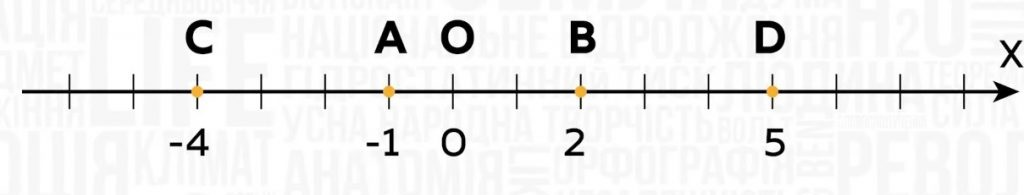
\includegraphics[align=t, width=\linewidth]{\picpath/G61M6C1-1}
			\end{minipage}
			\begin{minipage}[c]{0.45\textwidth}
				Сравните координаты точек: 
				\begin{tasks}(6)
					\task \( C \) и \( O \),
					\task \( A \) и \( O \),
					\task \( C \) и \( A \),
					\task \( D \) и \( C \),
					\task \( A \) и \( B \),
					\task \( A \) и \( D \).
				\end{tasks}
			\end{minipage}
		\item Сравните:
		\begin{tasks}(3)
			\task \( -2 \) .. \( 0 \)
			\task \( -3 \) .. \( -1 \)
			\task \( -5 \) .. \( -7 \)
			\task \( -13 \) .. \( -14 \)
			\task \( -21 \) .. \( -12 \)
			\task \( -1,5 \) .. \( -7 \)
			\task \( -2,3 \) .. \( -3 \)
			\task \( -3,5 \) .. \( -4,1 \)
			\task \( -8,25 \) .. \( -8,05 \)
			\task \( -2,2 \) .. \( -2,205 \)
			\task \( -\dfrac{1}{3} \) .. \( -\dfrac{2}{3} \)
			\task \( -\dfrac{7}{5} \) .. \( -\dfrac{4}{5} \)
			\task \( -\mfrac{4}{5}{6} \) .. \( -\mfrac{4}{7}{12} \)
			\task \( -\dfrac{5}{4} \) .. \( -1,1 \)
			\task \( -\dfrac{9}{10} \) .. \( -0,8 \)
		\end{tasks}
		\item Вычислите и сравните результаты:
		\begin{tasks}(1)
			\task \( 0,6-12,5 \)  и  \( 11,7-23,5 \)
			\task \( \mfrac{5}{7}{10}-4 \) и \( -25,3 +\dfrac{12}{5} \)
			\task \( -1,18+\dfrac{33}{50} \) и \( -0.3 + (-2,1) \)
			\task \( -25-\dfrac{3}{4} \) и \(-\dfrac{11}{10}-24,11\)
			\task \( \dfrac{7}{8}-\dfrac{11}{4} \) и \( -\dfrac{5}{8}-11 \)
		\end{tasks}
		\item Из \(225\) кг руды получили \(34,2\) кг меди. Каково процентное содержание меди в руде?
	\end{listofex}
	\newpage
	\title{Домашняя работа}
	\begin{listofex}
		\item
		%\hspace{0.02\linewidth}
		\begin{minipage}[c]{0.45\textwidth}
			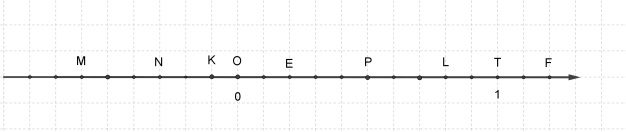
\includegraphics[align=t, width=\linewidth]{\picpath/G61M6L1-1}
		\end{minipage}
		\begin{minipage}[c]{0.45\textwidth}
			Сравните координаты точек: 
			\begin{tasks}(3)
				\task \( M \) и \( P \),
				\task \( N \) и \( M \),
				%\task \( K \) и \( N \),
				%\task \( E \) и \( O \),
				%\task \( M \) и \( E \),
				\task \( N \) и \( K \).
			\end{tasks}
		\end{minipage}
		\item Сравните:
		\begin{tasks}(3)
			\task \( -5 \) .. \( -3 \)
			%\task \( -4 \) .. \( -7 \)
			%\task \( -3 \) .. \( -3,5 \)
			%\task \( -1,5 \) .. \( -2,2 \)
			\task \( -4,5 \) .. \( -4 \)
			%\task \( -10,5 \) и \( -1,5 \)
			%\task \( -8,9 \) и \( -9,2 \)
			\task \( -55,3 \) и \( -55,4 \)
			\task \( -4,1 \) .. \( -4,2 \)
			%\task \( -\dfrac{7}{6} \) .. \( -7 \)
			\task \( -\dfrac{3}{8} \) .. \( -\dfrac{5}{8} \)
			\task \( -\mfrac{1}{2}{3} \) .. \( -\mfrac{1}{3}{4} \)
		\end{tasks}
		\item Вычислите и сравните результаты:
		\begin{tasks}(1)
			\task \( -11,2+4,12 \)  и  \( -0,7-7,2 \)
			\task \( \mfrac{3}{1}{5}-13 \) и \( -16,32 +\dfrac{27}{4} \)
			\task \( -\dfrac{3}{5}-\dfrac{13}{3} \) и \( -\dfrac{6}{5}-\mfrac{3}{2}{3} \)
		\end{tasks}
	\item Какова концентрация соли в растворе, состоящем из \(35\) г соли и \(165\) г воды?
	\end{listofex}
	\end{consultation}
%END_FOLD}